\documentclass[11pt,a4paper]{article}
\usepackage{../ma362}
\usepackage{tikz}
\usetikzlibrary{decorations.markings}
\usetikzlibrary{math,calc,arrows.meta}

\semester{Fall}
\year{2019}
\subtitlenumber{10}
\author{刘逸灏 (515370910207)}
\newcommand{\res}[1]{\mathop{\Res}\limits_{#1}}

\begin{document}
\maketitle

\section{六(一)/4}
\begin{problem}
求下列各积分之值:
\begin{enumerate}
  \item $\displaystyle\int_0^{2\pi}\frac{d\theta}{a+\cos\theta}\quad(a>1)$;
  \item $\displaystyle\int_0^{2\pi}\frac{dx}{(2+\sqrt{3}\cos x)^2}$.
\end{enumerate}
\end{problem}
\subsection*{(1)}
令$z=e^{i\theta}$, 则$d\theta=\dfrac{dz}{iz}$
$$\int_0^{2\pi}\frac{d\theta}{2a+\cos\theta}=\int_{|z|=1}\frac{2dz}{iz(a+z+z^{-1})}=\frac{2}{i}\int_{|z|=1}\frac{1}{z^2+2az+1}dz,$$
$$f(z)=\frac{1}{z^2+2az+1}=\frac{1}{(z+a-\sqrt{a^2-1})(z+a+\sqrt{a^2-1})}.$$
$-a+\sqrt{a^2-1}$为一阶极点, $-a-\sqrt{a^2-1}$为一阶极点, 只有$-a+\sqrt{a^2-1}$在圆$|z|<1$内.
$$\res{z=-a+\sqrt{a^2-1}}f(z)=\left.\frac{1}{z+a+\sqrt{a^2-1}}\right|_{z=-a+\sqrt{a^2-1}}=\frac{1}{2\sqrt{a^2-1}}.$$

由留数定理得
$$\int_0^{2\pi}\frac{d\theta}{2a+\cos\theta}=\frac{2}{i}\cdot 2\pi i\cdot \frac{1}{2\sqrt{a^2-1}}=\frac{2\pi}{\sqrt{a^2-1}}.$$

\subsection*{(2)}
令$z=e^{ix}$, 则$dx=\dfrac{dz}{iz}$
$$\int_0^{2\pi}\frac{dx}{(2+\sqrt{3}\cos x)^2}=\int_{|z|=1}\frac{4dz}{iz(4+\sqrt{3}z+\sqrt{3}z^{-1})^2}=\frac{4}{i}\int_{|z|=1}\frac{z}{(\sqrt{3}z^2+4z+\sqrt{3})^2}dz,$$
$$f(z)=\frac{z}{(\sqrt{3}z^2+4z+\sqrt{3})^2}=\frac{z}{(z+\sqrt{3})^2(\sqrt{3}z+1)^2}.$$
$-\sqrt{3}$为二阶极点, $-\dfrac{1}{\sqrt{3}}$为二阶极点, 只有$-\dfrac{1}{\sqrt{3}}$在圆$|z|<1$内.
$$\res{z=-\frac{1}{\sqrt{3}}}f(z)=\left.\left[\frac{z}{3(z+\sqrt{3})^2}\right]'\right|_{z=-\frac{1}{\sqrt{3}}}=\left.\frac{\sqrt{3}-z}{3(\sqrt{3}+z)^3}\right|_{z=-\frac{1}{\sqrt{3}}}=\frac{1}{2}.$$

由留数定理得
$$\int_0^{2\pi}\frac{dx}{(2+\sqrt{3}\cos x)^2}=\frac{4}{i}\cdot 2\pi i\cdot \frac{1}{2}=4\pi.$$

\section{六(一)/5}
\begin{problem}
求下列各积分:
\begin{enumerate}
  \addtocounter{enumi}{1}
  \item $\displaystyle\int_{-\infty}^{+\infty}\frac{x^2}{(x^2+a^2)^2}dx\quad(a>0)$;
        \addtocounter{enumi}{1}
  \item $\displaystyle\int_0^{+\infty}\frac{x\sin mx}{x^4+a^4}dx\quad(m>0,a>0)$.
\end{enumerate}
\end{problem}
\subsection*{(2)}
$$f(z)=\frac{z^2}{(z^2+a^2)^2}=\frac{z^2}{(z-ia)^2(z+ia)^2}.$$
$ia$为二阶极点, $-ia$为二阶极点, 只有$ia$在上半平面内.
$$\res{z=ia}=\left.\left[\frac{z^2}{(z+ia)^2}\right]'\right|_{z=ia}=\left.-\frac{2az}{(a-iz)^3}\right|_{z=ia}=-\frac{i}{4a}.$$
由定理6.7得
$$\frac{x^2}{(x^2+a^2)^2}dx=2\pi i\cdot-\frac{i}{4a}=\frac{\pi}{2a}.$$

\subsection*{(4)}
被积函数是偶函数, 故
$$\int_0^{+\infty}\frac{x\sin mx}{x^4+a^4}dx=\frac{1}{2}\int_{-\infty}^{+\infty}\frac{x\sin mx}{x^4+a^4}dx,$$
$$f(z)=\frac{ze^{imz}}{z^4+a^4}.$$
有四个一阶极点
$$a_k=ae^{\frac{\pi+2k\pi}{4}i},\quad (k=0,1,2,3),$$
$$\res{z=a_k}f(z)=\left.\frac{ze^{imz}}{(z^4+a^4)'}\right|_{z=a_k}=\left.\frac{e^{imz}}{4z^2}\right|_{z=a_k}=\frac{e^{ima_k}}{4a_k^2}.$$
$f(z)$在上半平面内只有两个极点$a_0$和$a_1$
$$\res{z=a_0}f(z)=\frac{e^{-\frac{\sqrt{2}ma}{2}+i\frac{\sqrt{2}ma}{2}}}{4a^2i}=\frac{e^{-\frac{\sqrt{2}ma}{2}}}{4a^2i}\left(\cos\frac{\sqrt{2}ma}{2}+i\sin\frac{\sqrt{2}ma}{2}\right),$$
$$\res{z=a_1}f(z)=\frac{e^{-\frac{\sqrt{2}ma}{2}-i\frac{\sqrt{2}ma}{2}}}{-4a^2i}=-\frac{e^{-\frac{\sqrt{2}ma}{2}}}{4a^2i}\left(\cos\frac{\sqrt{2}ma}{2}-i\sin\frac{\sqrt{2}ma}{2}\right).$$
由定理6.8得
$$\int_{-\infty}^{+\infty}\frac{xe^{imx}}{x^4+a^4}dx=2\pi i\cdot \left[\res{z=a_0}f(z)+\res{z=a_1}f(z)\right]=2\pi i\cdot \frac{e^{-\frac{\sqrt{2}ma}{2}}}{4a^2i}\cdot 2i\sin\frac{\sqrt{2}ma}{2}=i\frac{\pi}{a^2} e^{-\frac{\sqrt{2}ma}{2}}\sin\frac{\sqrt{2}ma}{2}.$$
且
$$\int_{-\infty}^{+\infty}\frac{xe^{imx}}{x^4+a^4}dx=\int_{-\infty}^{+\infty}\frac{x\cos mx}{x^4+a^4}dx+i\int_{-\infty}^{+\infty}\frac{x\sin mx}{x^4+a^4}dx.$$
故
$$\int_0^{+\infty}\frac{x\sin mx}{x^4+a^4}dx=\frac{\pi}{2a^2} e^{-\frac{\sqrt{2}ma}{2}}\sin\frac{\sqrt{2}ma}{2}.$$

\section{六(一)/6}
\begin{problem}
仿照例6.15的方法计算下列积分:
\begin{enumerate}
  \item $\displaystyle\int_0^{+\infty}\frac{\sin x}{x(x^2+a^2)}dx\quad(a>0)$;
  \item $\displaystyle\int_0^{+\infty}\frac{\sin x}{x(x^2+1)^2}dx$.
\end{enumerate}
\end{problem}
\subsection*{(1)}
被积函数是偶函数, 故
$$\int_0^{+\infty}\frac{\sin x}{x(x^2+a^2)}dx=\frac{1}{2}\text{P.V.}\int_{-\infty}^{+\infty}\frac{\sin x}{x(x^2+a^2)}dx,$$
$$f(z)=\frac{e^{iz}}{z(z^2+a^2)}=\frac{e^{iz}}{z(z-ia)(z+ia)}.$$
$0$为一阶极点, $ia$为一阶极点, $-ia$为一阶极点, 只有$ia$在上半平面内.
$$\res{z=ia}=\left.\frac{e^{iz}}{z(z+ia)}\right|_{z=ia}=-\frac{e^{-a}}{2a^2}.$$
考虑$f(z)$在上半平面内沿下图所示之闭曲线路径$C$的积分.
\begin{center}
  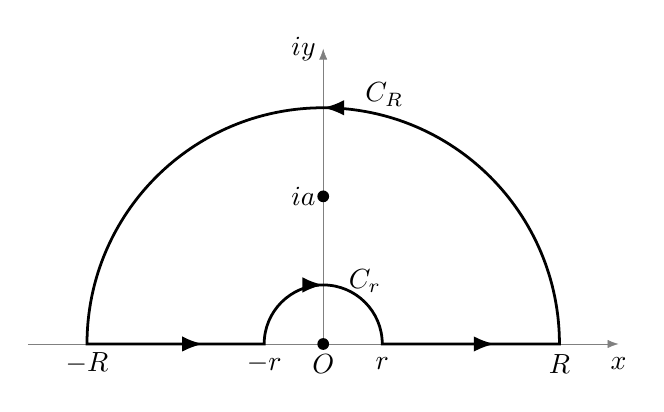
\begin{tikzpicture}[>/.tip={Latex}]
    % The axes
    \tikzmath{\r=0.75;\R=3;\a=0.5*\r+0.5*\R;}
    \draw[help lines,->] (-1.25*\R,0) -- (1.25*\R,0) coordinate (xaxis);
    \draw[help lines,->] (0,0) -- (0,1.25*\R) coordinate (yaxis);
    % The integral path
    \draw[
      line width=1pt,
      decoration={
          markings,
          mark=at position 0 with {\arrow{>}},
          mark=at position 0.16 with {\arrow{>}},
          mark=at position 0.5 with {\arrow{>}},
          mark=at position 0.88 with {\arrow{>}},
        },
      postaction={decorate}
    ] (0,\r) arc(90:0:\r) -- (\r,0)
    -- (\R,0) arc(0:180:\R) -- (-\R,0) 
    -- (-\r,0) arc(180:90:\r) -- cycle;
    
    \node at (-\r,-0.25) {$-r$};
    \node at (\r,-0.25) {$r$};
    \node at (-\R,-0.25) {$-R$};
    \node at (\R,-0.25) {$R$};
    \node at (0,-0.25) {$O$};
    \node[circle,fill,inner sep=1.5pt] at (0,0) {};
    \node at (-0.25,\a) {$ia$};
    \node[circle,fill,inner sep=1.5pt] at (0,\a) {};
    \node at (1.25*\R,-0.25) {$x$};
	\node at (-0.25,1.25*\R) {$iy$};
	\node[above] at (45:\r) {$C_r$};
	\node[above] at (75:\R) {$C_R$};
  \end{tikzpicture}
\end{center}
由留数定理得
$$\int_r^Rf(x)dx+\int_{C_R}f(z)dz+\int_{-R}^{-r}f(x)dx-\int_{C_r}f(z)dz=2\pi i\res{z=ia}=2\pi i\cdot -\frac{e^{-a}}{2a^2}=-i\pi\frac{e^{-a}}{a^2}.$$
由引理6.2知
$$\lim_{R\to+\infty}\int_{C_R}f(z)dz=\lim_{R\to+\infty}\int_{C_R}\frac{e^{iz}}{z(z^2+a^2)}dz=0.$$
由引理6.3知
$$\lim_{r\to0}\int_{C_r}f(z)dz=\lim_{r\to0}\int_{C_r}\frac{e^{iz}}{z(z^2+a^2)}dz=i\pi\lim_{r\to0}\frac{e^{iz}}{z^2+a^2}=i\pi\frac{1}{a^2}.$$
另$r\to0$, $R\to+\infty$可得
$$\text{P.V.}\int_{-\infty}^{+\infty}\frac{e^{ix}}{x(x^2+a^2)}dx=i\pi\frac{1-e^{-a}}{a^2}.$$
且
$$\int_{-\infty}^{+\infty}\frac{e^{ix}}{x(x^2+a^2)}dx=\int_{-\infty}^{+\infty}\frac{\cos x}{x(x^2+a^2)}dx+i\int_{-\infty}^{+\infty}\frac{\sin x}{x(x^2+a^2)}dx.$$
故
$$\int_0^{+\infty}\frac{\sin x}{x(x^2+a^2)}dx=\frac{\pi(1-e^{-a})}{2a^2}.$$
\subsection*{(2)}
被积函数是偶函数, 故
$$\int_0^{+\infty}\frac{\sin x}{x(x^2+1)^2}dx=\frac{1}{2}\text{P.V.}\int_{-\infty}^{+\infty}\frac{\sin x}{x(x^2+1)^2}dx,$$
$$f(z)=\frac{e^{iz}}{z(z^2+1)^2}=\frac{e^{iz}}{z(z-i)^2(z+i)^2}.$$
$0$为一阶极点, $i$为二阶极点, $-i$为二阶极点, 只有$i$在上半平面内.
$$\res{z=i}=\left.\left[\frac{e^{iz}}{z(z+i)^2}\right]'\right|_{z=i}=\left.\frac{ie^{iz}(z^2+4iz-1)}{z^2(z+i)^3}\right|_{z=i}=-\frac{3}{4e}.$$
考虑$f(z)$在上半平面内沿下图所示之闭曲线路径$C$的积分.
\begin{center}
  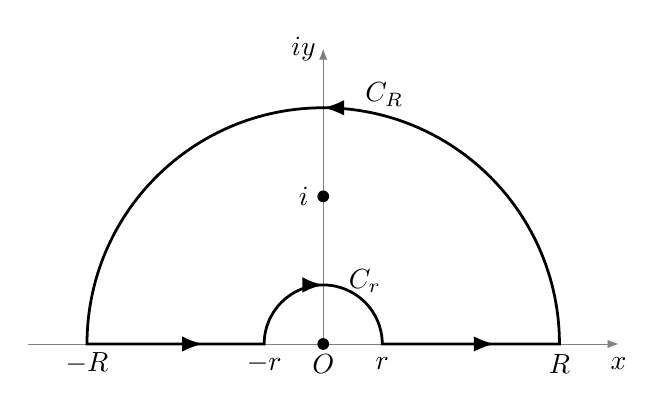
\begin{tikzpicture}[>/.tip={Latex}]
    % The axes
    \tikzmath{\r=0.75;\R=3;\a=0.5*\r+0.5*\R;}
    \draw[help lines,->] (-1.25*\R,0) -- (1.25*\R,0) coordinate (xaxis);
    \draw[help lines,->] (0,0) -- (0,1.25*\R) coordinate (yaxis);
    % The integral path
    \draw[
      line width=1pt,
      decoration={
          markings,
          mark=at position 0 with {\arrow{>}},
          mark=at position 0.16 with {\arrow{>}},
          mark=at position 0.5 with {\arrow{>}},
          mark=at position 0.88 with {\arrow{>}},
        },
      postaction={decorate}
    ] (0,\r) arc(90:0:\r) -- (\r,0)
    -- (\R,0) arc(0:180:\R) -- (-\R,0) 
    -- (-\r,0) arc(180:90:\r) -- cycle;
    
    \node at (-\r,-0.25) {$-r$};
    \node at (\r,-0.25) {$r$};
    \node at (-\R,-0.25) {$-R$};
    \node at (\R,-0.25) {$R$};
    \node at (0,-0.25) {$O$};
    \node[circle,fill,inner sep=1.5pt] at (0,0) {};
    \node at (-0.25,\a) {$i$};
    \node[circle,fill,inner sep=1.5pt] at (0,\a) {};
    \node at (1.25*\R,-0.25) {$x$};
	\node at (-0.25,1.25*\R) {$iy$};
	\node[above] at (45:\r) {$C_r$};
	\node[above] at (75:\R) {$C_R$};
  \end{tikzpicture}
\end{center}
由留数定理得
$$\int_r^Rf(x)dx+\int_{C_R}f(z)dz+\int_{-R}^{-r}f(x)dx-\int_{C_r}f(z)dz=2\pi i\res{z=ia}=2\pi i\cdot -\frac{3}{4e}=-i\pi\frac{3}{2e}.$$
由引理6.2知
$$\lim_{R\to+\infty}\int_{C_R}f(z)dz=\lim_{R\to+\infty}\int_{C_R}\frac{e^{iz}}{z(z^2+1)^2}dz=0.$$
由引理6.3知
$$\lim_{r\to0}\int_{C_r}f(z)dz=\lim_{r\to0}\int_{C_r}\frac{e^{iz}}{z(z^2+1)^2}dz=i\pi\lim_{r\to0}\frac{e^{iz}}{(z^2+1)^2}=i\pi.$$
另$r\to0$, $R\to+\infty$可得
$$\text{P.V.}\int_{-\infty}^{+\infty}\frac{e^{ix}}{x(x^2+1)^2}dx=i\pi\left(1-\frac{3}{2e}\right).$$
且
$$\int_{-\infty}^{+\infty}\frac{e^{ix}}{x(x^2+1)^2}dx=\int_{-\infty}^{+\infty}\frac{\cos x}{x(x^2+1)^2}dx+i\int_{-\infty}^{+\infty}\frac{\sin x}{x(x^2+1)^2}dx.$$
故
$$\int_0^{+\infty}\frac{\sin x}{x(x^2+1)^2}dx=\pi\left(\frac{1}{2}-\frac{3}{4e}\right).$$
\end{document}
